\documentclass[tikz,border=6pt]{standalone}
\usepackage{amsmath,amssymb}
\usepackage{tikz}
\usetikzlibrary{decorations.pathmorphing, decorations.markings, arrows.meta}
\begin{document}
% 调节 scale 可以整体放大缩小
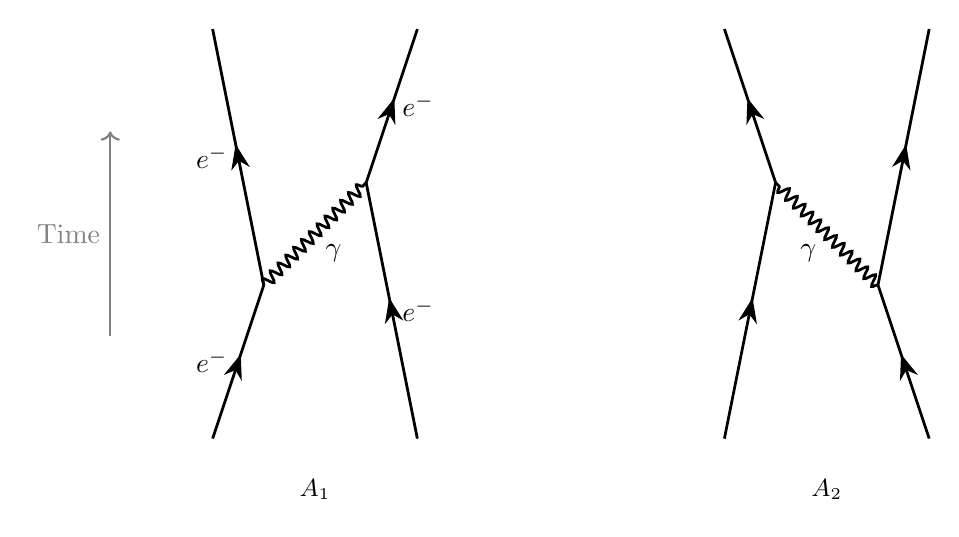
\begin{tikzpicture}[scale=1.3, line width=1pt,
    % --- 样式定义 ---
    photon/.style={decorate, decoration={snake, amplitude=2pt, segment length=4pt}},
    fermion/.style={postaction={decorate},
        decoration={markings,mark=at position 0.55 with {\arrow{Stealth[scale=1.2]}}}},
    label_text/.style={font=\small} % 字体大小
]

    % =========================================
    % 【左图：图 (a)】 左边电子先发射光子
    % 整体向左平移 2.5 单位
    % =========================================
    \begin{scope}[shift={(-2.5, 0)}]
        
        % --- 1. 定义坐标 (折线逻辑) ---
        % 左路电子：从下(-1) -> 往里折(-0.5) -> 往外弹(-1)
        % 注意 v_L (顶点) 的 Y 是 -0.5 (较早/较低)
        \coordinate (L_in)  at (-1.0, -2.0);
        \coordinate (L_v)   at (-0.5, -0.5); % 左顶点：低
        \coordinate (L_out) at (-1.0,  2.0);

        % 右路电子：从下(1) -> 往里折(0.5) -> 往外弹(1)
        % 注意 v_R (顶点) 的 Y 是 0.5 (较晚/较高)
        \coordinate (R_in)  at ( 1.0, -2.0);
        \coordinate (R_v)   at ( 0.5,  0.5); % 右顶点：高
        \coordinate (R_out) at ( 1.0,  2.0);

        % --- 2. 连线 ---
        % 左电子流
        \draw[fermion] (L_in) -- (L_v) node[midway, left] {$e^-$};
        \draw[fermion] (L_v) -- (L_out) node[midway, left] {$e^-$};
        
        % 右电子流
        \draw[fermion] (R_in) -- (R_v) node[midway, right] {$e^-$};
        \draw[fermion] (R_v) -- (R_out) node[midway, right] {$e^-$};

        % 交换光子 (左低 -> 右高)
        \draw[photon] (L_v) -- (R_v) node[midway, below right] {$\gamma$};
        
        % 图注
        \node[label_text] at (0, -2.5) {$A_1$};
    \end{scope}

    % =========================================
    % 【右图：图 (b)】 右边电子先发射光子
    % 整体向右平移 2.5 单位
    % =========================================
    \begin{scope}[shift={(2.5, 0)}]

        % --- 1. 定义坐标 ---
        % 注意这里 Y 坐标的反转
        
        % 左路电子：顶点变高了 (Y=0.5)
        \coordinate (L_in_2)  at (-1.0, -2.0);
        \coordinate (L_v_2)   at (-0.5,  0.5); % 左顶点：高 (晚)
        \coordinate (L_out_2) at (-1.0,  2.0);

        % 右路电子：顶点变低了 (Y=-0.5)
        \coordinate (R_in_2)  at ( 1.0, -2.0);
        \coordinate (R_v_2)   at ( 0.5, -0.5); % 右顶点：低 (早)
        \coordinate (R_out_2) at ( 1.0,  2.0);

        % --- 2. 连线 ---
        \draw[fermion] (L_in_2) -- (L_v_2);
        \draw[fermion] (L_v_2) -- (L_out_2);
        
        \draw[fermion] (R_in_2) -- (R_v_2);
        \draw[fermion] (R_v_2) -- (R_out_2);

        % 交换光子 (右低 -> 左高)
        \draw[photon] (R_v_2) -- (L_v_2) node[midway, below left] {$\gamma$};

        % 图注
        \node[label_text] at (0, -2.5) {$A_2$};
    \end{scope}

    % --- 可选：画个时间轴在最左边 ---
    \draw[->, thick, gray] (-4.5, -1) -- (-4.5, 1) node[midway, left] {Time};

\end{tikzpicture}
\end{document}
